\chapter{Context Viewpoint Template} \label{chp:context-viewpoint-template}
	\begin{comment}
		The Context viewpoint depicts services provided by a design subject with reference to an explicit context.
		That context is defined by reference to actors that include users and other stakeholders, which interact with
		the design subject in its environment. The Context viewpoint provides a “black box” perspective on the
		design subject.
		Services depict an inherently functional aspect or anticipated cases of use of the design subject (hence “use
		cases” in UML). Stratification of services and their descriptions in the form of scenarios of actors’
		interactions with the system provide a mechanism for adding detail. Services may also be associated with
		actors through information flows. The content and manner of information exchange with the environment
		implies additional design information and the need for additional viewpoints (see 5.10).
		A Deployment overlay to a Context view can be transformed into a Deployment view whenever the
		execution hardware platform is part of the design subject; for stand-alone software design, a Deployment
		overlay maps software entities onto externally available entities not subject of the current design effort.
		Similarly, work allocation to teams and other management perspectives are overlays in the design.
	\end{comment}
	This viewpoint identifies basic features of \emph{Computational Library}, main user and example of input data.
	\section{Design concerns} \label{s:context-viewpoint-template:design-concerns}
		\begin{comment}
			The purpose of the Context viewpoint is to identify a design subject’s offered services, its actors (users and
			other interacting stakeholders), to establish the system boundary and to effectively delineate the design
			subject’s scope of use and operation.
			Drawing a boundary separating a design subject from its environment, determining a set of services to be
			provided, and the information flows between design subject and its environment, is typically a key design
			decision. That makes this viewpoint applicable to most design efforts.
			When the system is portrayed as a black box, with internal decisions hidden, the Context view is often a
			starting point of design, showing what is to be designed functionally as the only available information
			about the design subject: a name and an associated set of externally identifiable services. Requirements
			analysis identifies these services with the specification of quality of service attributes, henceforth invoking
			many non-functional requirements. Frequently incomplete, a Context view is begun in requirements
			analysis. Work to complete this view continues during design.
		\end{comment}
		
		\begin{concerns}{Library use--cases}{API}
			\begin{figure}[!htp]
				\centering
				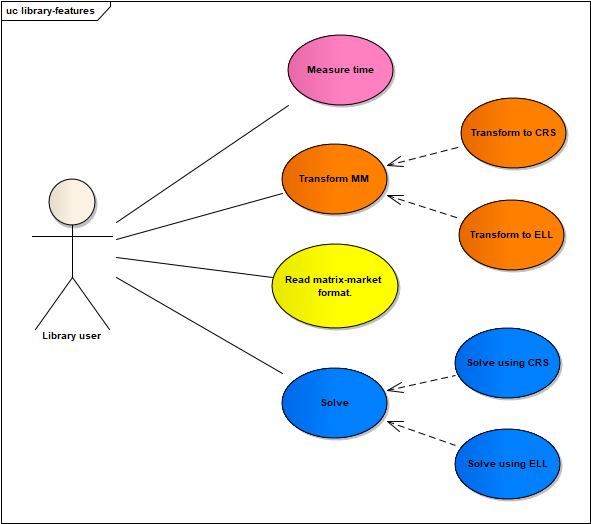
\includegraphics[scale=0.6]{others/img/library-features}
				\caption{Use--case diagram of computation library features.}
			\end{figure}
		\end{concerns}
		\clearpage
		\begin{concerns}{Example \gls{MM} file}{Input}
			\lstinputlisting[basicstyle=\tiny]{others/cage4.mtx}
		\end{concerns}
		\clearpage
		\begin{concerns}{Basic usage of library features}{API}
			\begin{figure}[!htp]
				\centering
				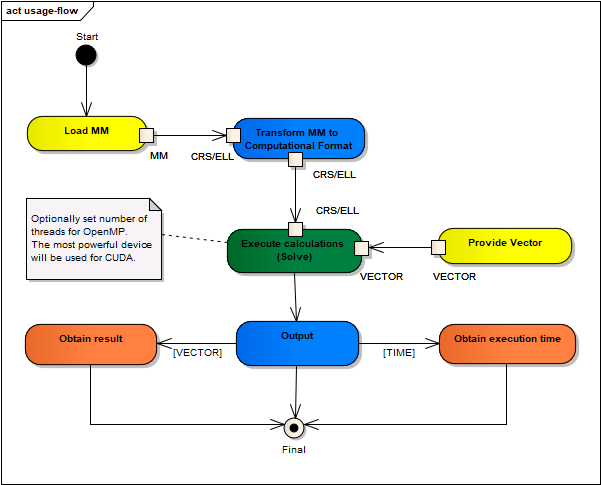
\includegraphics[scale=0.6]{others/img/usage-flow}
				\caption{General usage--flow of application.}
			\end{figure}
		\end{concerns}
	\section{Design elements} \label{s:context-viewpoint-template:design-elements}
		\begin{comment}
			Design entities: actors—external active elements interacting with the design subject, including users, other
			stakeholders and external systems, or other items; services—also called use cases; and directed information
			flows between the design subject, treated as a black box, and its actors associating actors with services.
			Flows capture the expected information content exchanged.
			
			Design relationships: receive output and provide input (between actors and the design subject).
			
			Design constraints: qualities of service; form and medium of interaction (provided to and received from)
			with environment.
		\end{comment}
	
		\begin{design-element}{User}{Actor}
			User of the library can be a programmer, researcher or scientist.
		\end{design-element}
	
		\begin{design-element}{\gls{MM} file}{Constraints}
			Following storage-data types are supported:
			\begin{itemize}
				\item general
				\item symmetric
			\end{itemize}
			Following value data types are supported:
			\begin{itemize}
				\item real
				\item pattern
				\item integer
			\end{itemize}
		\end{design-element}
	%\section{Example languages} \label{s:context-viewpoint-template:example-languages}
		\begin{comment}
			Any black-box type diagrams can be used to realize the Context viewpoint. Appropriate languages include
			Structured Analysis [e.g., IDEF0 (IEEE Std 1320.1-1998 [B18]), Structured Analysis and Design 
			Technique (SADT) (Ross [B32]) or those of the DeMarco or Gane-Sarson variety], the Cleanroom’s black
			box diagrams, and UML use cases (OMG [B28]).
		\end{comment}